\providecommand\ExamFontPath{../../../字体/}
\documentclass[fontset=exam]{exam-zh}
\usepackage{longtable,booktabs,array,calc,multirow,fvextra}
\usepackage[normalem]{ulem}
\providecommand{\hl}[1]{#1}
\providecommand{\ul}[1]{\uline{#1}}
\DefineVerbatimEnvironment{verbatim}{Verbatim}{breaklines=true,fontsize=\small}
\providecommand{\tightlist}{\setlength{\itemsep}{0pt}\setlength{\parskip}{0pt}}
\newcommand{\pandocbounded}[1]{#1}
\setlength{\emergencystretch}{3em}
\setlength{\tabcolsep}{2pt}
\examsetup{page/size=a4paper}
\title{厦门大学 2018—2019 年 期末考试 A 卷}
\subject[4em]{概率统计}
\setcounter{tocdepth}{1}
\begin{document}
\maketitle
\fancyfoot[C]{第 \thepage 页（共 \pageref*{LastPage} 页）}
\begin{enumerate}
\item
  选择题（在各小题四个备选答案中选出一个正确答案，填在题末的括号中，本大题共 6 个小题，每小题 3 分，总计 18 分）
\end{enumerate}

\begin{enumerate}
\def\labelenumi{\arabic{enumi}.}
\item
  已知随机变量\(X_1,X_2,\ldots,X_n\)相互独立，且都在区间（-1，1）上服从均匀分布，由独立同分布中心极限定理， \(\lim_{n\to\infty}p\left(\sum_{i=1}^n X_i<\sqrt n\right)=\)\underline{\hspace{2cm}}
\end{enumerate}

\begin{enumerate}
\def\labelenumi{\Alph{enumi}.}
\item
  \(\Phi(\sqrt3)\) B. \(\Phi\left(\sqrt{\frac13}\right)\) C. \(\Phi(3)\) D. \(\Phi\left(\frac13\right)\)
\end{enumerate}

\begin{enumerate}
\def\labelenumi{\arabic{enumi}.}
\setcounter{enumi}{1}
\item
  设 \(X_1,X_2,\ldots,X_9\)服从同一分布，\(E(X_i)=1,D(X_i)=1\)，对于任意的 \(\varepsilon>0\)有（ ）
\end{enumerate}

\begin{quote}
A.\(P\left\{\left|\sum_{i=1}^9X_i-1\right|<\varepsilon\right\}\geq1-\frac1{\varepsilon^2}\) B.\(P\left\{\left|\frac19\sum_{i=1}^9X_i-1\right|<\varepsilon\right\}\geq1-\frac1{9\varepsilon^2}\)

C.\(P\left\{\left|\frac19\sum_{i=1}^9X_i-9\right|<\varepsilon\right\}\geq1-\frac1{9\varepsilon^2}\) D. \(P\left\{\left|\sum_{i=1}^9X_i-9\right|<\varepsilon\right\}\geq1-\frac1{\varepsilon^2}\)
\end{quote}

\begin{enumerate}
\def\labelenumi{\arabic{enumi}.}
\setcounter{enumi}{2}
\item
  设\(X_1,X_2,\ldots,X_n\ (n\geq2)\)是来自标准正态总体的简单随机样本，\(\overline X\)为样本均值，\(S^2\)为样本方差，则（ ）
\end{enumerate}

\begin{quote}
A \(n\overline X\sim N(0,1)\) B \(nS^2\sim\chi^2(n)\)

C \(\frac{(n-1)\overline X}{S}\sim t(n-1)\) D \(\frac{(n-1)X_1^2}{\sum_{i=2}^nX_i^2}\sim F(1,n-1)\)
\end{quote}

\begin{enumerate}
\def\labelenumi{\arabic{enumi}.}
\setcounter{enumi}{3}
\item
  设\(X_1,X_2,\ldots,X_n\)是取自总体\(X\)的一个随机样本， \(E(X)=\mu,D(X)=\sigma^2\), \(\widehat\theta^2=C\sum_{i=1}^{n-1}(X_{i+1}-X_i)^2\)为\(\sigma^2\)的无偏估计，则\(C=\)（ ）
\end{enumerate}

\begin{quote}
A．\(1/n\) B. \(1/(n-1)\)

C. \(1/2(n-1)\) D. \(1/(n-2)\)
\end{quote}

\begin{enumerate}
\def\labelenumi{\arabic{enumi}.}
\setcounter{enumi}{4}
\item
  设\(X_1,X_2,\ldots,X_n\)是取自总体\(X\)的一个简单样本，则\(E(X^2)\)的矩估计是（ ）
\end{enumerate}

\begin{quote}
A．\(\frac1{n-1}\sum_{i=1}^n(X_i-\overline X)^2+\overline X\) B. \(\frac1n\sum_{i=1}^n(X_i-\overline X)^2+\overline X\)

C. \(\frac1{n-1}\sum_{i=1}^n(X_i-\overline X)^2+\overline X^2\) D. \(\frac1n\sum_{i=1}^n(X_i-\overline X)^2+\overline X^2\)
\end{quote}

\begin{enumerate}
\def\labelenumi{\arabic{enumi}.}
\setcounter{enumi}{5}
\item
  在假设检验中,下列说法错误的是 ( ) .
\end{enumerate}

A. \(H_1\)为真时拒绝\(H_1\)称为犯第二类错误.

B. \(H_1\)不真时接受\(H_1\)称为犯第一类错误.

C. 设 P\{拒绝\(H_0\mid H_0\)为真\}=\(\alpha\), P\{接受\(H_0\mid H_0\)不真\}=\(\beta\),则\(\alpha\)变大时\(\beta\)变小.

D. \(\alpha\),\(\beta\)的意义同 (C), 当样本容量一定时, \(\alpha\)变大时则\(\beta\)变小.

\pdfbookmark[1]{二、填空题}{section17}

\par\medskip{\heiti

二、填空题（本大题共 6 小题，每小题 3 分，总计 18 分）

\par}\smallskip

\begin{enumerate}
\def\labelenumi{\arabic{enumi}.}
\item
  已知某产品的次品率为 0.04，现有一批产品 100 件，求这批产品中不少于 4 件次品的概率\underline{\hspace{2cm}}。
\item
  设\(X_1,X_2,\ldots,X_n\ (n>1)\)是来自总体的简单随机样本，且其方差为\(\sigma^2>0\)，令\(Y=\frac1n\sum_{i=1}^nX_i\)，则\(\operatorname{Cov}(X_1,Y)=\)\underline{\hspace{2cm}}。
\item
  设总体\(X\sim b(n,p)\)，\(0<p<1\)，\(X_1,X_2,\ldots,X_n\)为其样本，则\(n\)和\(p\)的矩估计量分别是\underline{\hspace{2cm}}、\underline{\hspace{2cm}}。
\item
  设总体\(X\sim U(0,\theta)\)，\(X_1,X_2,\ldots,X_n\)为其样本，则\(\theta\)的最大似然估计量是\underline{\hspace{2cm}}。
\item
  某大学从来自 A、B 两市的新生中分别随机抽取 5 名与 6 名新生，测其身高（单位：cm）后算的\(\overline x=175.9,\overline y=172.0;s_1^2=11.3,s_2^2=9.1\)。假设两市新生身高分别服从正态分布\(X\sim N(\mu_1,\sigma^2),Y\sim N(\mu_2,\sigma^2)\)，其中\(\sigma^2\)未知。\(\mu_1-\mu_2\)的置信度为 0.95 的单侧置信上限为\underline{\hspace{2cm}}。
\item
  设总体\(X:N(\mu_1,\sigma_1^2)\)，\(Y:N(\mu_2,\sigma_2^2)\)检验假设\(H_0:\sigma_1^2=\sigma_2^2\)，显著性水平\(\alpha=0.1\)，从 X,Y 中分别抽取样本容量为\(n_1=12,n_2=10\)的样本，算得\(S_1^2=118.4,S_2^2=31.93\)，则正确的检验应用\underline{\hspace{2cm}}检验法，\underline{\hspace{2cm}}（接受/拒绝）\(H_0\)。
\end{enumerate}

\pdfbookmark[1]{三、解答题}{section19}

三、（10 分）保险公司有 10000 人参加保险，每人每年付 12 元保险费，在一年内一个人生病概率为 0.006，患者可以向保险公司领得 1000 元赔偿

（1）保险公司亏本的概率多大?

\begin{quote}
（2）保险公司一年利润不少于 60000 元概率？
\end{quote}

\pdfbookmark[1]{四、解答题}{section22}

四、（14 分）设\(X_1,X_2,\ldots,X_n\ (n\geq2)\)是来自标准总体的简单随机样本，\(\overline X\)为样本均值，记\(Y_i=X_i-\overline X,i=1,2,\ldots,n\)

\begin{quote}
求：（1）\(Y_i\)的方差\(D(Y_i),i=1,2,\ldots,n\)
\end{quote}

\begin{enumerate}
\def\labelenumi{\arabic{enumi}.}
\setcounter{enumi}{1}
\item
  \(Y_1\)与\(Y_n\)的协方差\(\operatorname{Cov}(Y_1,Y_n)\)
\end{enumerate}

\pdfbookmark[1]{五、解答题}{section25}

五、（8 分）设总体的概率密度函数为 \(f(x) = \left\{ \begin{array}{l}
{\text{3}\lambda x^{2}e^{- \lambda x^{3}},x > 0} \\
{0\text{,}\text{其它}}
\end{array} \right.\) ，其中\(\lambda>0\)是未知参数，\(x_1,x_2,\ldots,x_n\)是一组样本值，求参数\(\lambda\)的最大似然估计。

\pdfbookmark[1]{六、解答题}{section26}

六、（10 分）某车间生产滚珠，可认为滚珠的直径服从正态分布，且直径的方差为\(\sigma^2=0.04\)，从某天生产的产品中随机抽取 9 个，测得直径平均值为 15mm。试对\(\alpha=0.05\)求出滚珠的平均直径的区间估计。

\pdfbookmark[1]{七、解答题}{section27}

七、（12 分）某食品厂用自动装罐机装罐头食品, 规定标准重量为 250 克, 标准差不超过 3 克时机器工作为正常, 每天定时检验机器情况, 现抽取 16 罐, 测得平均重量\(\overline X=252\)克, 样本标准差\(S=4\)克, 假定罐头重量服从正态分布, 试问该机器工作是否正常? (显著性水平为 0.05)

\pdfbookmark[1]{八、解答题}{section28}

八、（10 分）设\(\{X_n\}\)是独立同分布的随机变量序列，且假设\(E[X_n]=2,D[X_n]=6\)证明：

\[\frac{X_1^2+X_2X_3+X_4^2+X_5X_6+\cdots+X_{3n-2}^2+X_{3n-1}X_{3n}}n\xrightarrow{n\to\infty}a\]

并确定\(a\)的值。

\newpage
附表： \(\Phi(x) = {\int_{- \infty}^{x}{\frac{1}{\sqrt{2\pi}}e^{- \frac{t^{2}}{2}}dt}}\)

\begin{longtable}[]{@{}
  >{\centering\arraybackslash}p{(\linewidth - 20\tabcolsep) * \real{0.0563}}
  >{\centering\arraybackslash}p{(\linewidth - 20\tabcolsep) * \real{0.0944}}
  >{\centering\arraybackslash}p{(\linewidth - 20\tabcolsep) * \real{0.0944}}
  >{\centering\arraybackslash}p{(\linewidth - 20\tabcolsep) * \real{0.0944}}
  >{\centering\arraybackslash}p{(\linewidth - 20\tabcolsep) * \real{0.0944}}
  >{\centering\arraybackslash}p{(\linewidth - 20\tabcolsep) * \real{0.0944}}
  >{\centering\arraybackslash}p{(\linewidth - 20\tabcolsep) * \real{0.0944}}
  >{\centering\arraybackslash}p{(\linewidth - 20\tabcolsep) * \real{0.0944}}
  >{\centering\arraybackslash}p{(\linewidth - 20\tabcolsep) * \real{0.0944}}
  >{\centering\arraybackslash}p{(\linewidth - 20\tabcolsep) * \real{0.0944}}
  >{\centering\arraybackslash}p{(\linewidth - 20\tabcolsep) * \real{0.0940}}@{}}
\toprule\noalign{}
\endhead
\bottomrule\noalign{}
\endlastfoot
\emph{x} & 0 & 0.01 & 0.02 & 0.03 & 0.04 & 0.05 & 0.06 & 0.07 & 0.08 & 0.09 \\
1 & 0.841 3 & 0.843 8 & 0.846 1 & 0.848 5 & 0.850 8 & 0.853 1 & 0.855 4 & 0.857 7 & 0.859 9 & 0.862 1 \\
1.1 & 0.864 3 & 0.866 5 & 0.868 6 & 0.870 8 & 0.872 9 & 0.874 9 & 0.877 0 & 0.879 0 & 0.881 0 & 0.883 0 \\
1.2 & 0.884 9 & 0.886 9 & 0.888 8 & 0.890 7 & 0.892 5 & 0.894 4 & 0.896 2 & 0.898 0 & 0.899 7 & 0.901 5 \\
1.3 & 0.903 2 & 0.904 9 & 0.906 6 & 0.908 2 & 0.909 9 & 0.911 5 & 0.913 1 & 0.914 7 & 0.916 2 & 0.917 7 \\
1.4 & 0.919 2 & 0.920 7 & 0.922 2 & 0.923 6 & 0.925 1 & 0.926 5 & 0.927 9 & 0.929 2 & 0.930 6 & 0.931 9 \\
& & & & & & & & & & \\
1.5 & 0.933 2 & 0.934 5 & 0.935 7 & 0.937 0 & 0.938 2 & 0.939 4 & 0.940 6 & 0.941 8 & 0.943 0 & 0.944 1 \\
1.6 & 0.945 2 & 0.946 3 & 0.947 4 & 0.948 4 & 0.949 5 & 0.950 5 & 0.951 5 & 0.952 5 & 0.953 5 & 0.953 5 \\
1.7 & 0.955 4 & 0.956 4 & 0.957 3 & 0.958 2 & 0.959 1 & 0.959 9 & 0.960 8 & 0.961 6 & 0.962 5 & 0.963 3 \\
1.8 & 0.964 1 & 0.964 8 & 0.965 6 & 0.966 4 & 0.967 2 & 0.967 8 & 0.968 6 & 0.969 3 & 0.970 0 & 0.970 6 \\
1.9 & 0.971 3 & 0.971 9 & 0.972 6 & 0.973 2 & 0.973 8 & 0.974 4 & 0.975 0 & 0.975 6 & 0.976 2 & 0.976 7 \\
& & & & & & & & & & \\
2 & 0.977 2 & 0.977 8 & 0.978 3 & 0.978 8 & 0.979 3 & 0.979 8 & 0.980 3 & 0.980 8 & 0.981 2 & 0.981 7 \\
2.1 & 0.982 1 & 0.982 6 & 0.983 0 & 0.983 4 & 0.983 8 & 0.984 2 & 0.984 6 & 0.985 0 & 0.985 4 & 0.985 7 \\
2.2 & 0.986 1 & 0.986 4 & 0.986 8 & 0.987 1 & 0.987 4 & 0.987 8 & 0.988 1 & 0.988 4 & 0.988 7 & 0.989 0 \\
2.3 & 0.989 3 & 0.989 6 & 0.989 8 & 0.990 1 & 0.990 4 & 0.990 6 & 0.990 9 & 0.991 1 & 0.991 3 & 0.991 6 \\
2.4 & 0.991 8 & 0.992 0 & 0.992 2 & 0.992 5 & 0.992 7 & 0.992 9 & 0.993 1 & 0.993 2 & 0.993 4 & 0.993 6 \\
\end{longtable}

F 分布：

\par\medskip{\centering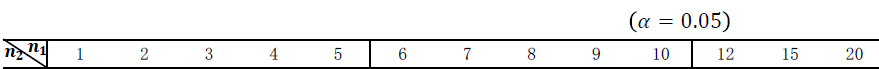
\includegraphics[width=15cm]{figures/image86.png}\par}\medskip

\par\medskip{\centering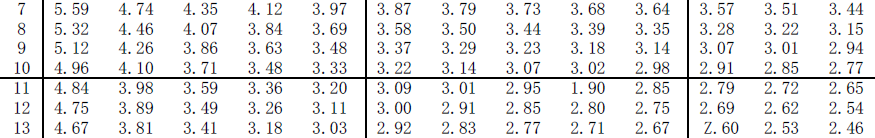
\includegraphics[width=15cm]{figures/image87.png}\par}\medskip

\par\medskip{\centering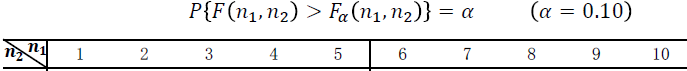
\includegraphics[width=15cm]{figures/image88.png}\par}\medskip \par\medskip{\centering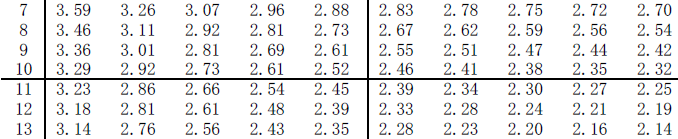
\includegraphics[width=15cm]{figures/image89.png}\par}\medskip

\noindent\begin{minipage}{\linewidth}
卡方分布：

\par\medskip{\centering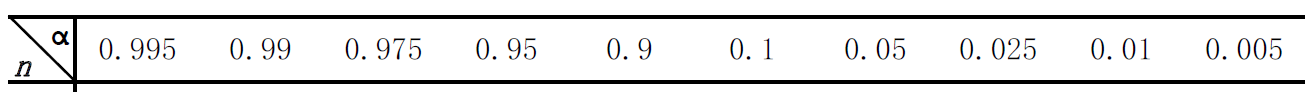
\includegraphics[width=15cm]{figures/image90.png}\par}\medskip

\par\medskip{\centering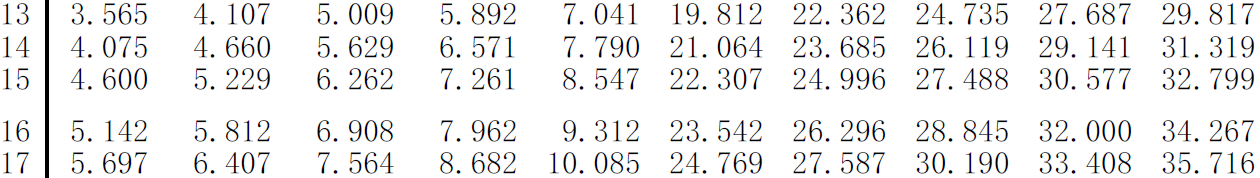
\includegraphics[width=15cm]{figures/image91.png}\par}\medskip
\end{minipage}

\noindent\begin{minipage}{\linewidth}
t 分布：

\par\medskip{\centering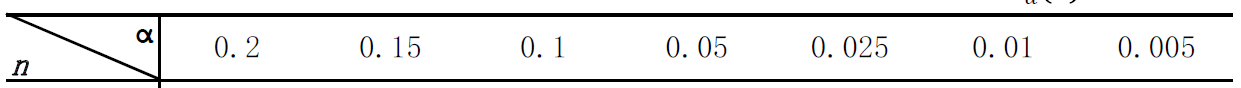
\includegraphics[width=15cm]{figures/image92.png}\par}\medskip

\par\medskip{\centering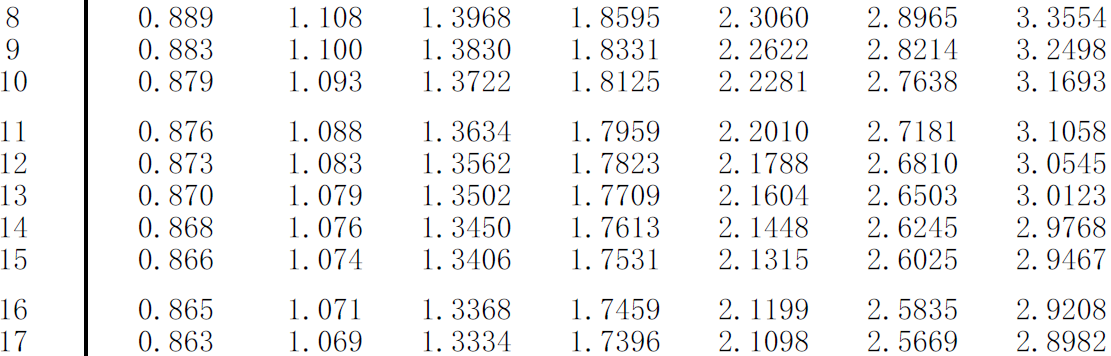
\includegraphics[width=15cm]{figures/image93.png}\par}\medskip
\end{minipage}

\end{document}
